\chapter{UXtweak}

\label{chap:UXtweak}


Uxtweak offers a number of different usability tests, as well as analysis tools.
Not only do they allow users to create card sorting studies, but also tree 
tests and replay tests on other websites. All of their products can be 
accessed for free, however there are a number of limitations that should entice
users to upgrade to a premium membership. This review will only focus on the
card sorting capabilities of UXtweak

\begin{figure}[tp] 
\centering
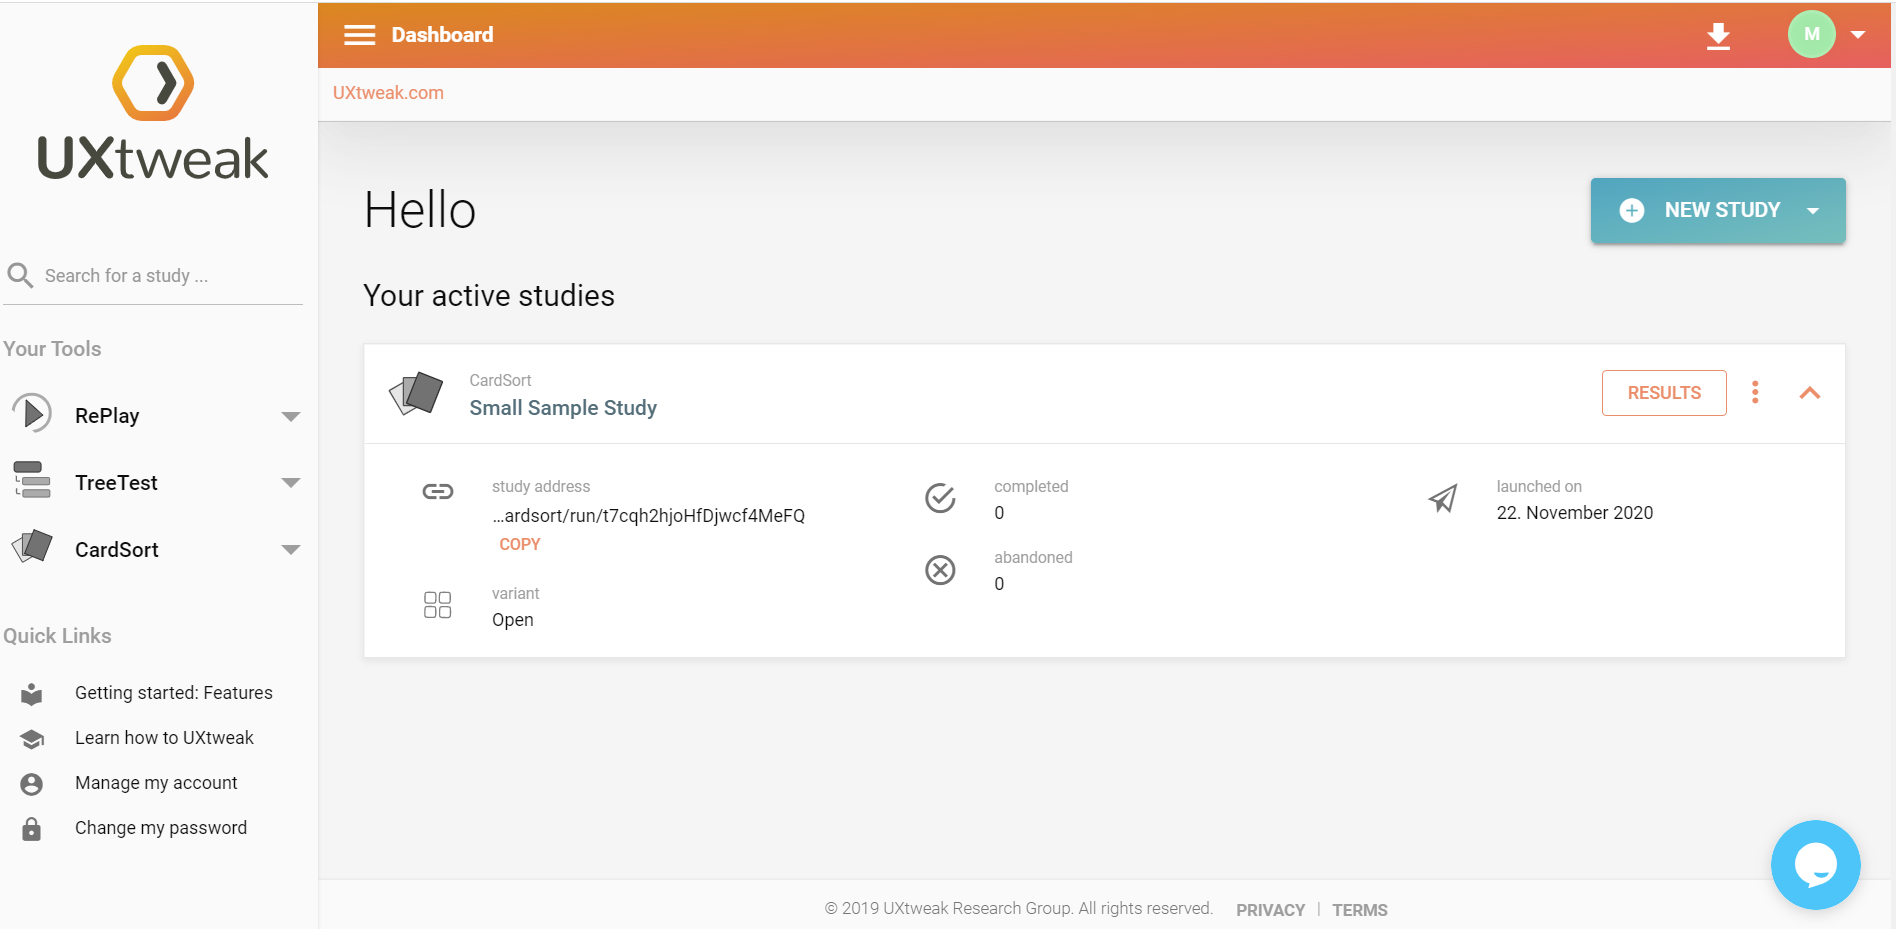
\includegraphics[keepaspectratio,width=\linewidth,height=\halfh]{images/uxtweak-dashboard.png}
\caption[UXtweak Application] { This is the base view in UXtweak.
It shows you the currently active studies in the center with some information 
such as the launch date and the study address link.
\imgcredit{Screenshot was captured byMarkus Ruplitsch using
\textcite{UXtweak} on Google Chrome 84.} }
\label{fig:UXtweak1}
\end{figure}

\section{Business Model}
As mentioned before, most of the offered features can be accessed for free after
 creating an account. However, there are  a number of restrictions when using a
free account. The most notable restriction is that the number of cards per card
sorting study is limited to 20 and the number of respondents is limited to 10 per
study. This means that, for most users who want to test larger navigation
structures, it is necessary to upgrade to a premium account in order to get 
unlimited cards and respondents per study. Additional features that a users gets
for purchasing a premium membership include: branding options, support and an
unlimited number of .pdf reports (instead of one every 48 hours).

Currently, the price for a monthly subscription is €140.- per month. 
Alternatively one can purchase a years worth of premium subscription for
€1,176.-. In case a more custom plan is required, they also advertise the 
option to contact them and negotiate a custom plan. It is also worth 
mentioning that UXtweak offers a 5-day free trial for their premium membership.
A screenshot of the dashboard can be seen in figure ~\ref{fig:UXtweak1}.

\section{Card Sorting}
The card sorting itself is  easy to set up, as UXtweaks menus are highly 
intuitive and their written documentation is extremely detailed. Once a user 
creates a new card sorting study, they are prompted to go through all the 
different customization options UXtweak has to offer. These options are 
structured in several different tabs and users can go back and forth between 
them in whichever order they prefer. At any point there is the option to look at
a preview of the study and, in case any field is unclear, there are little helper
icons that give a more detailed explanation about the information required. 
Overall there is an extensive number of different customization options,
especially when it comes to creating questionaires before or after the study. 

When using an account with a premium membership it is also possible to customize
the colors and style of the study, as well as include logos or other branding 
tools. After a study has been launched, participants can either enter via a URL 
link or by clicking a widget that can be copied from UXtweak and embedded in 
another website. A screenshot of the card sorting process can be seen in figure
~\ref{fig:UXtweak2}.

\begin{figure}[tp] 
\centering
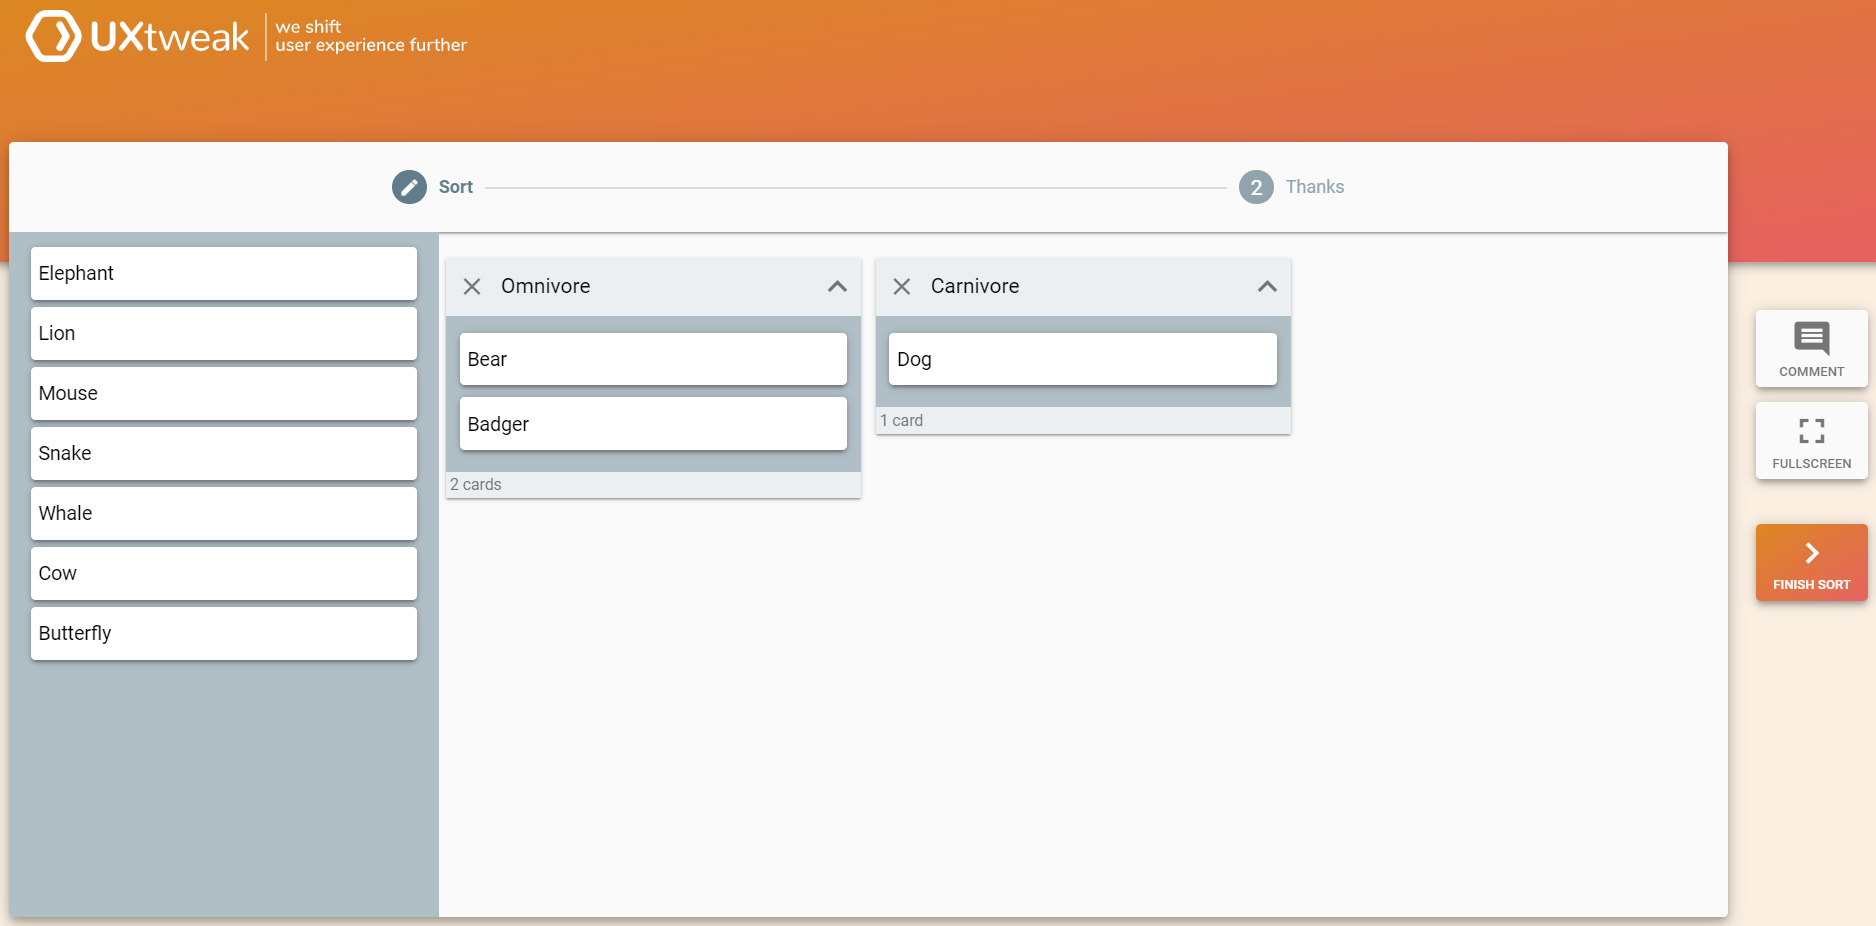
\includegraphics[keepaspectratio,width=\linewidth,height=\halfh]{images/uxtweak-sorting.png}
\caption[UXtweak Card Sorting] { This is a screenshot during the card
sorting process in UXtweak.
\imgcredit{Screenshot was captured by Markus Ruplitsch using
\textcite{UXtweak} on Google Chrome 84.} }
\label{fig:UXtweak2}
\end{figure}

\section{Analytics}
Even if the card sorting study has not yet concluded it is possible to view the 
current results and analytics online. UXtweaks study review shows information 
about the number of participants, their locations, time taken and how many 
cards they sorted. It is possible to filter or sort the participants and their 
information by any of these criteria, and to include or exclude them in the 
remaining analysis. Their analysis shows which cards have been sorted into 
which categories and vice versa. They offer a results matrix a similarity matrix
and participants can leave comments during their card sort that can late be 
reviewed. Additionally, they offer a dendrogram and a standardization grid.

All of these analytics can be exported as PDF (only one .pdf export every 48 
hours with a free plan) or CSV. Results can also be shared online via URL link 
and can be partially hidden to users with a URL link unless they have a 
password, which can be set manually. An overview of all features can be seen in
table ~\ref{tab:features-UXtweak}.

\begin{table}[tp]
\centering
\begin{tabularx}
{\linewidth}{|l|X|}
\hline \textbf{Feature/Characteristic} & \textbf{Availability in UXtweak} \\ 
\hline Card Sorting & Open, closed and hybrid. \\ 
\hline Card Limit & 20 with a free plan, unlimited with a premium plan. \\
\hline Participant Limit & 10 with a free plan, unlimited with a premium 
plan.\\
\hline Analytics & standardization grid, similarity matrix, dendrogram,
 respondent-centric analysis \\ 
\hline Documentation & Extremely detailed written documentation with a 
number of screenshots \\
\hline Business Model & Free or €140.- per month / €1176.- per year \\
\hline Import formats & .csv\\ 
\hline Export formats & .csv and .pdf, results can also be shared online \\ 
\hline Sub-Categories & No. \\ 
\hline Playback of user-sessions & No. \\ 
\hline Data preparation & Allows filtering and exclusion/includsion of specific
 users. \\ 
\hline
\end{tabularx} 
\caption[Feature summary of UXtweak] 
{ 
This table summarizes all the features and characteristics of UXtweak
to provide an easy to read overview.
}
\label{tab:features-UXtweak}
\end{table}


\section{Summary \& Ratings}
Because UXtweak is so easy to use and offers a detailed documentation it is 
possible to quickly create a card sorting study while still having a large 
number of customization options. The user interface is extremely friendly 
and the resulting study looks professional, even without including custom 
branding options. The analytics view offers a lot of different analysis tools 
and all results can be shared via a number of different ways. All in all, 
UXtweaks has a lot to offer when it comes to card sorting, even to non-paying 
users.

The only significant downside to using UXtweak is that the limitations that come
with using a free plan, make it impossible to conduct larger studies without 
upgrading to a premium membership. And, while there is a free trial, for €140.-
a month it might still be worth considering a different option.  The ratings can 
be found in table ~\ref{tab:rating-UXtweak} and range from 0-5.


\begin{table}[tp] 
\centering 
\begin{tabularx}{\linewidth}{|X|X|X|X|X|}
\hline
Simplicity & Documentation & Features & Business Model & Average \\ 
\hline 
5 & 4 & 4 & 3 & 4.0 \\ 
\hline 
\end{tabularx} 
\caption[Ratings for UXtweak] {
Ratings for UXtweak including the average rating.
} 
\label{tab:rating-UXtweak}
\end{table}





